\section{Оценки коэффициентов дисторсии}
\begin{table}[H]
	\centering
	\begin{tabular}{| c | c | c | c| c | }
		\hline
		& $\lambda_1$ & Ошибка на инлаер & Число инлаеров\\ \hline
		A & -0.7549144 & 2.5              & 400 \\ \hline
		B & -0.7908241  & 2.9              & 100  \\ \hline
		C & -0.832088 & 2.8              & 1200 \\ 
		\hline
	\end{tabular}
	\caption{Усредненные (относительно всех пар) результаты автоматического решателя}
\end{table}

\begin{table}[H]
	\centering
	\begin{tabular}{| c | c | c | c| c | }
		\hline
		& $\lambda_1$ & $\lambda_2$ & Ошибка на инлаер &  Число инлаеров \\ \hline
		A & -0.722611 & -0.104535 & 1.55 & 4054 \\ \hline
		B &  -0.756474 & -0.0270121  & 2.24 & 1906  \\ \hline
		C & -0.736565 & -0.163169 & 1.66 & 11305 \\ 
		\hline
	\end{tabular}
	\caption{Оценки коэффициентов дисторсии и ошибка на инлаер после оптимизации фундаментальной матрицы}
\end{table}

\begin{table}[H]
	\centering
	\begin{tabular}{| c | c | c | c| c | }
		\hline 
		& $\lambda_1$ & $\lambda_2$ & Ошибка на инлаер &  Число инлаеров \\ \hline
		A & -0.653171 & -0.25638 & 1.42 & 4338 \\ \hline
		B & -0.674782 & -0.256507 & 2.48 & 2005  \\ \hline
		C & -0.679329 & -0.273404 & 1.77 & 6346 \\ 
		\hline
	\end{tabular}
	\caption{Оценки коэффициентов дисторсии и ошибка на инлаер после совместной оптимизации}
\end{table}
Очень много соответствий для камеры C провалили тест хиральности, поэтому количество инлаеров сильно уменьшилось. Для камеры B существует много неправильных соответствий, так как на изображениях очень много схожих элементов (здание имеет периодический рельеф), поэтому средняя ошибка для нее больше.
\subsection{Примеры распрямленных изображений}
\begin{figure}[H]
	\centering 
	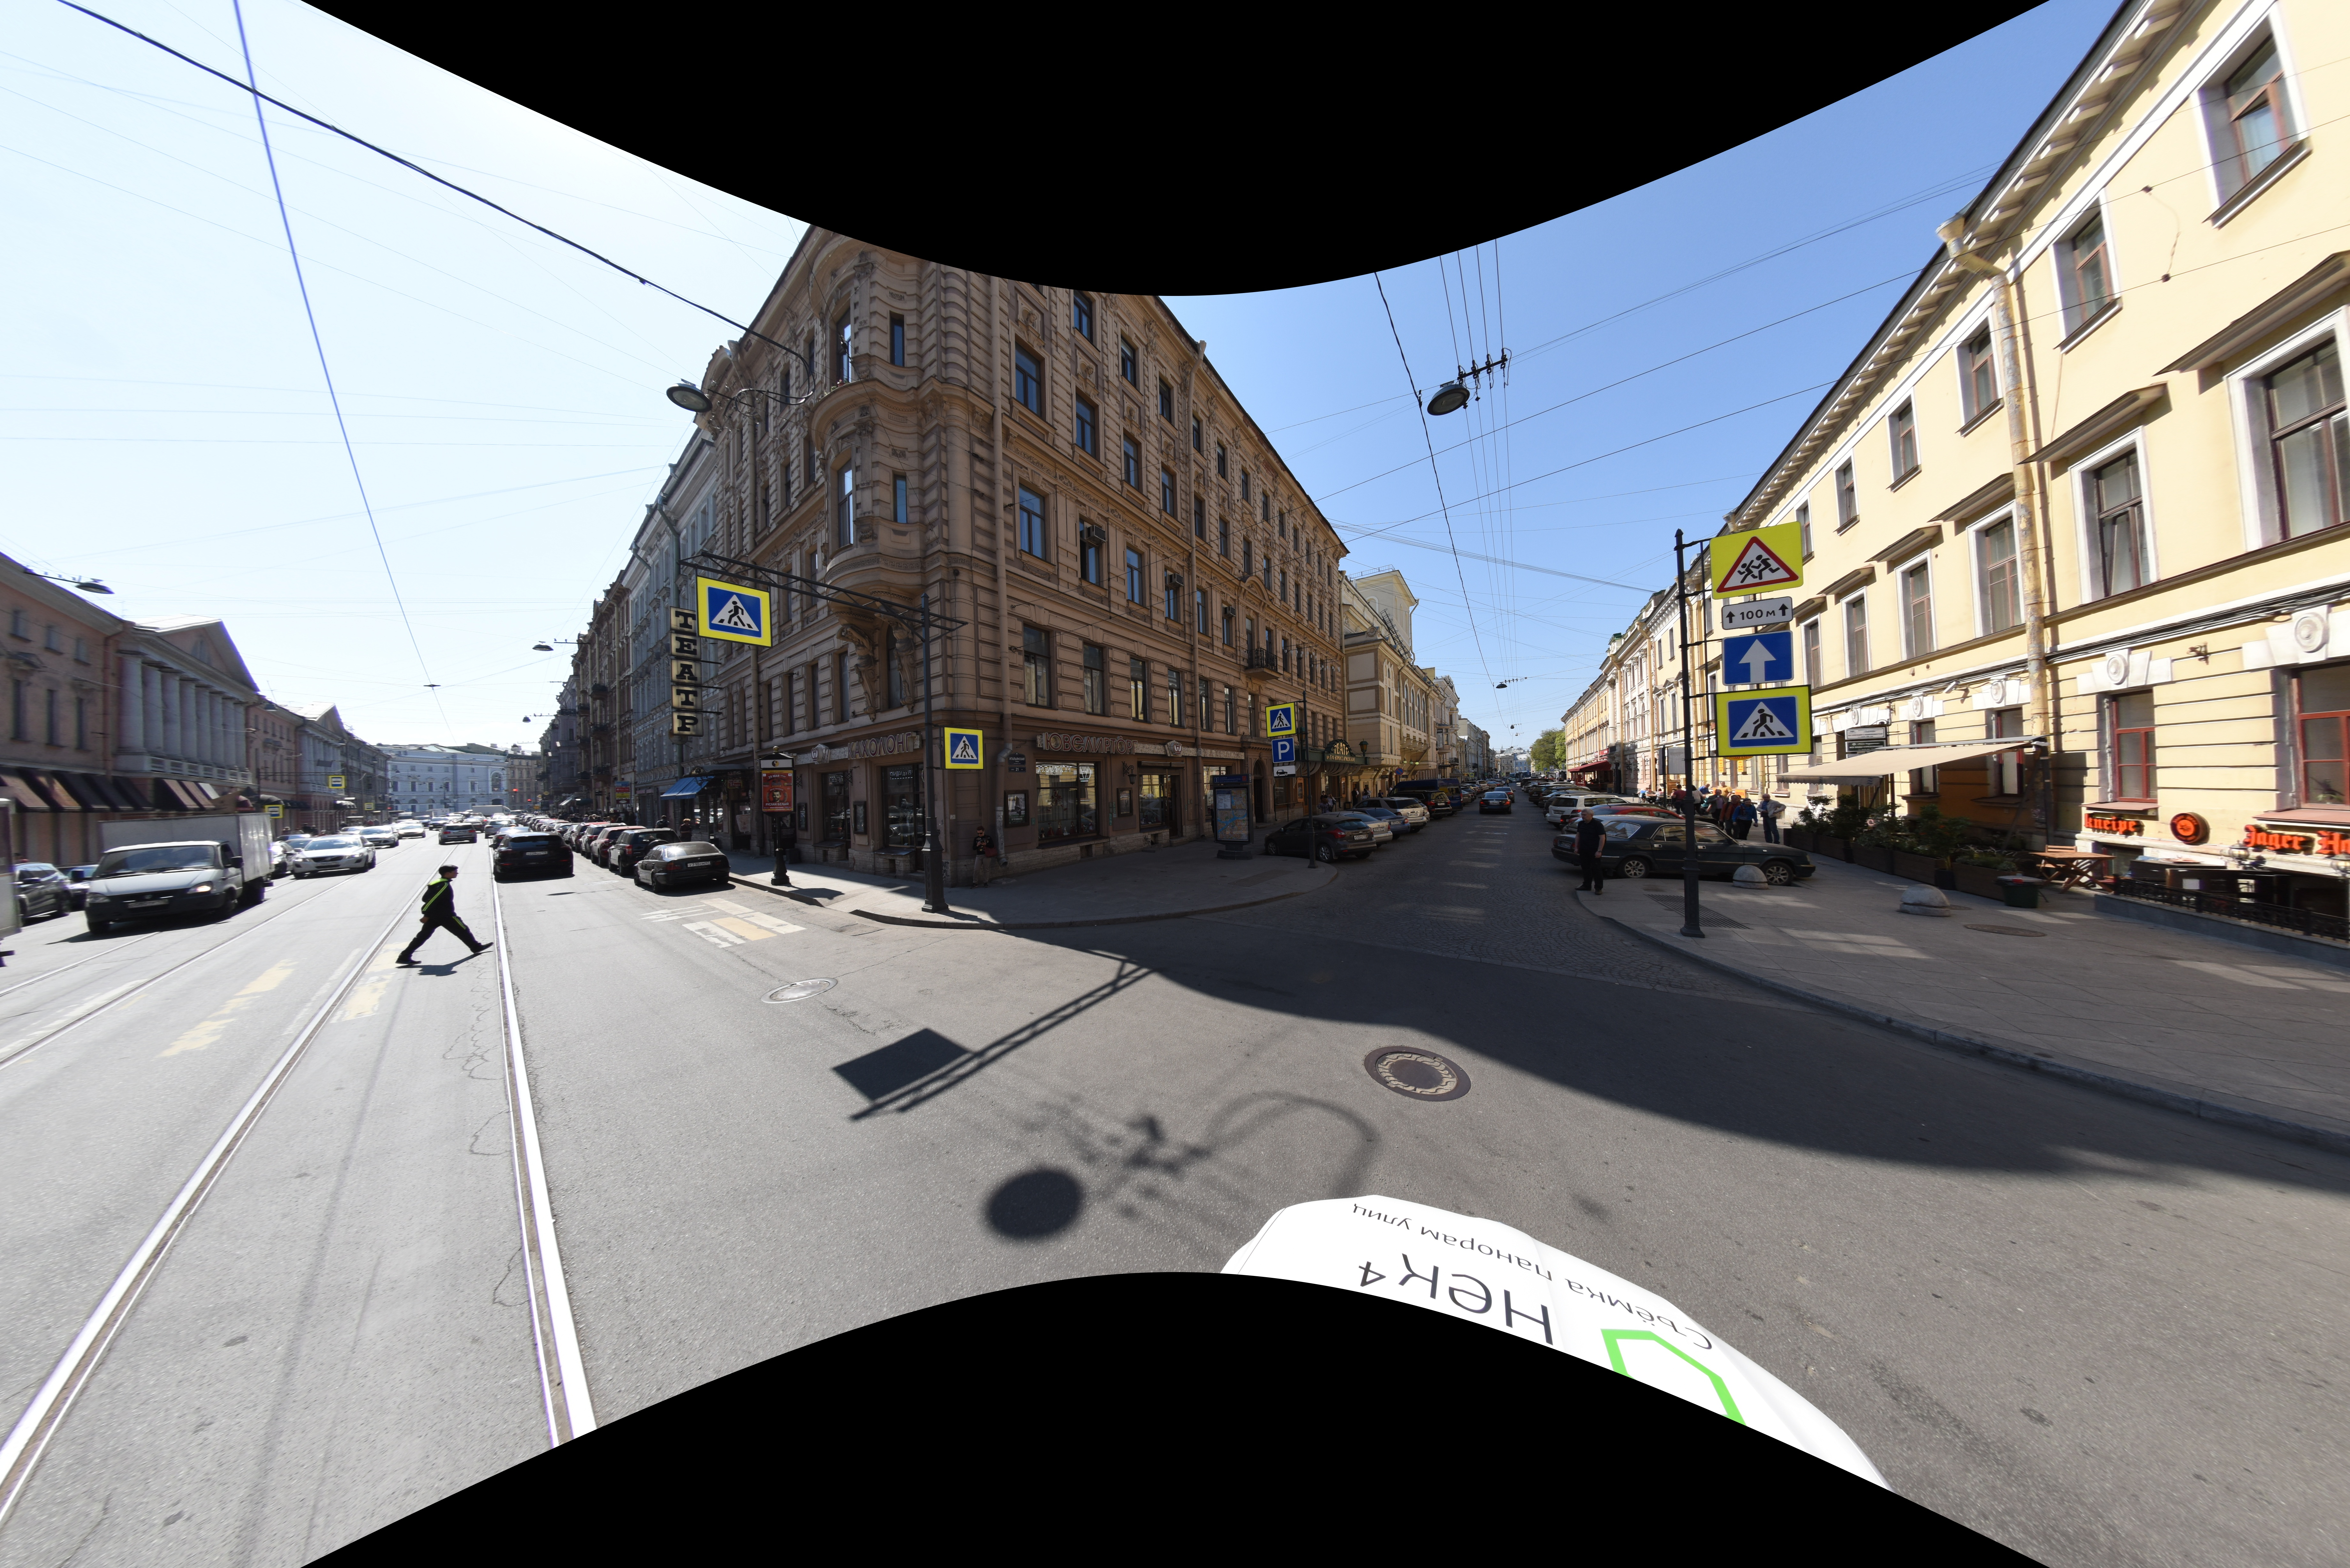
\includegraphics[width=0.9\textwidth]{figures/undistortedA552.JPG}
	\caption{A552 с одним коэффициентом}
\end{figure}
\begin{figure}[H]
	\centering 
	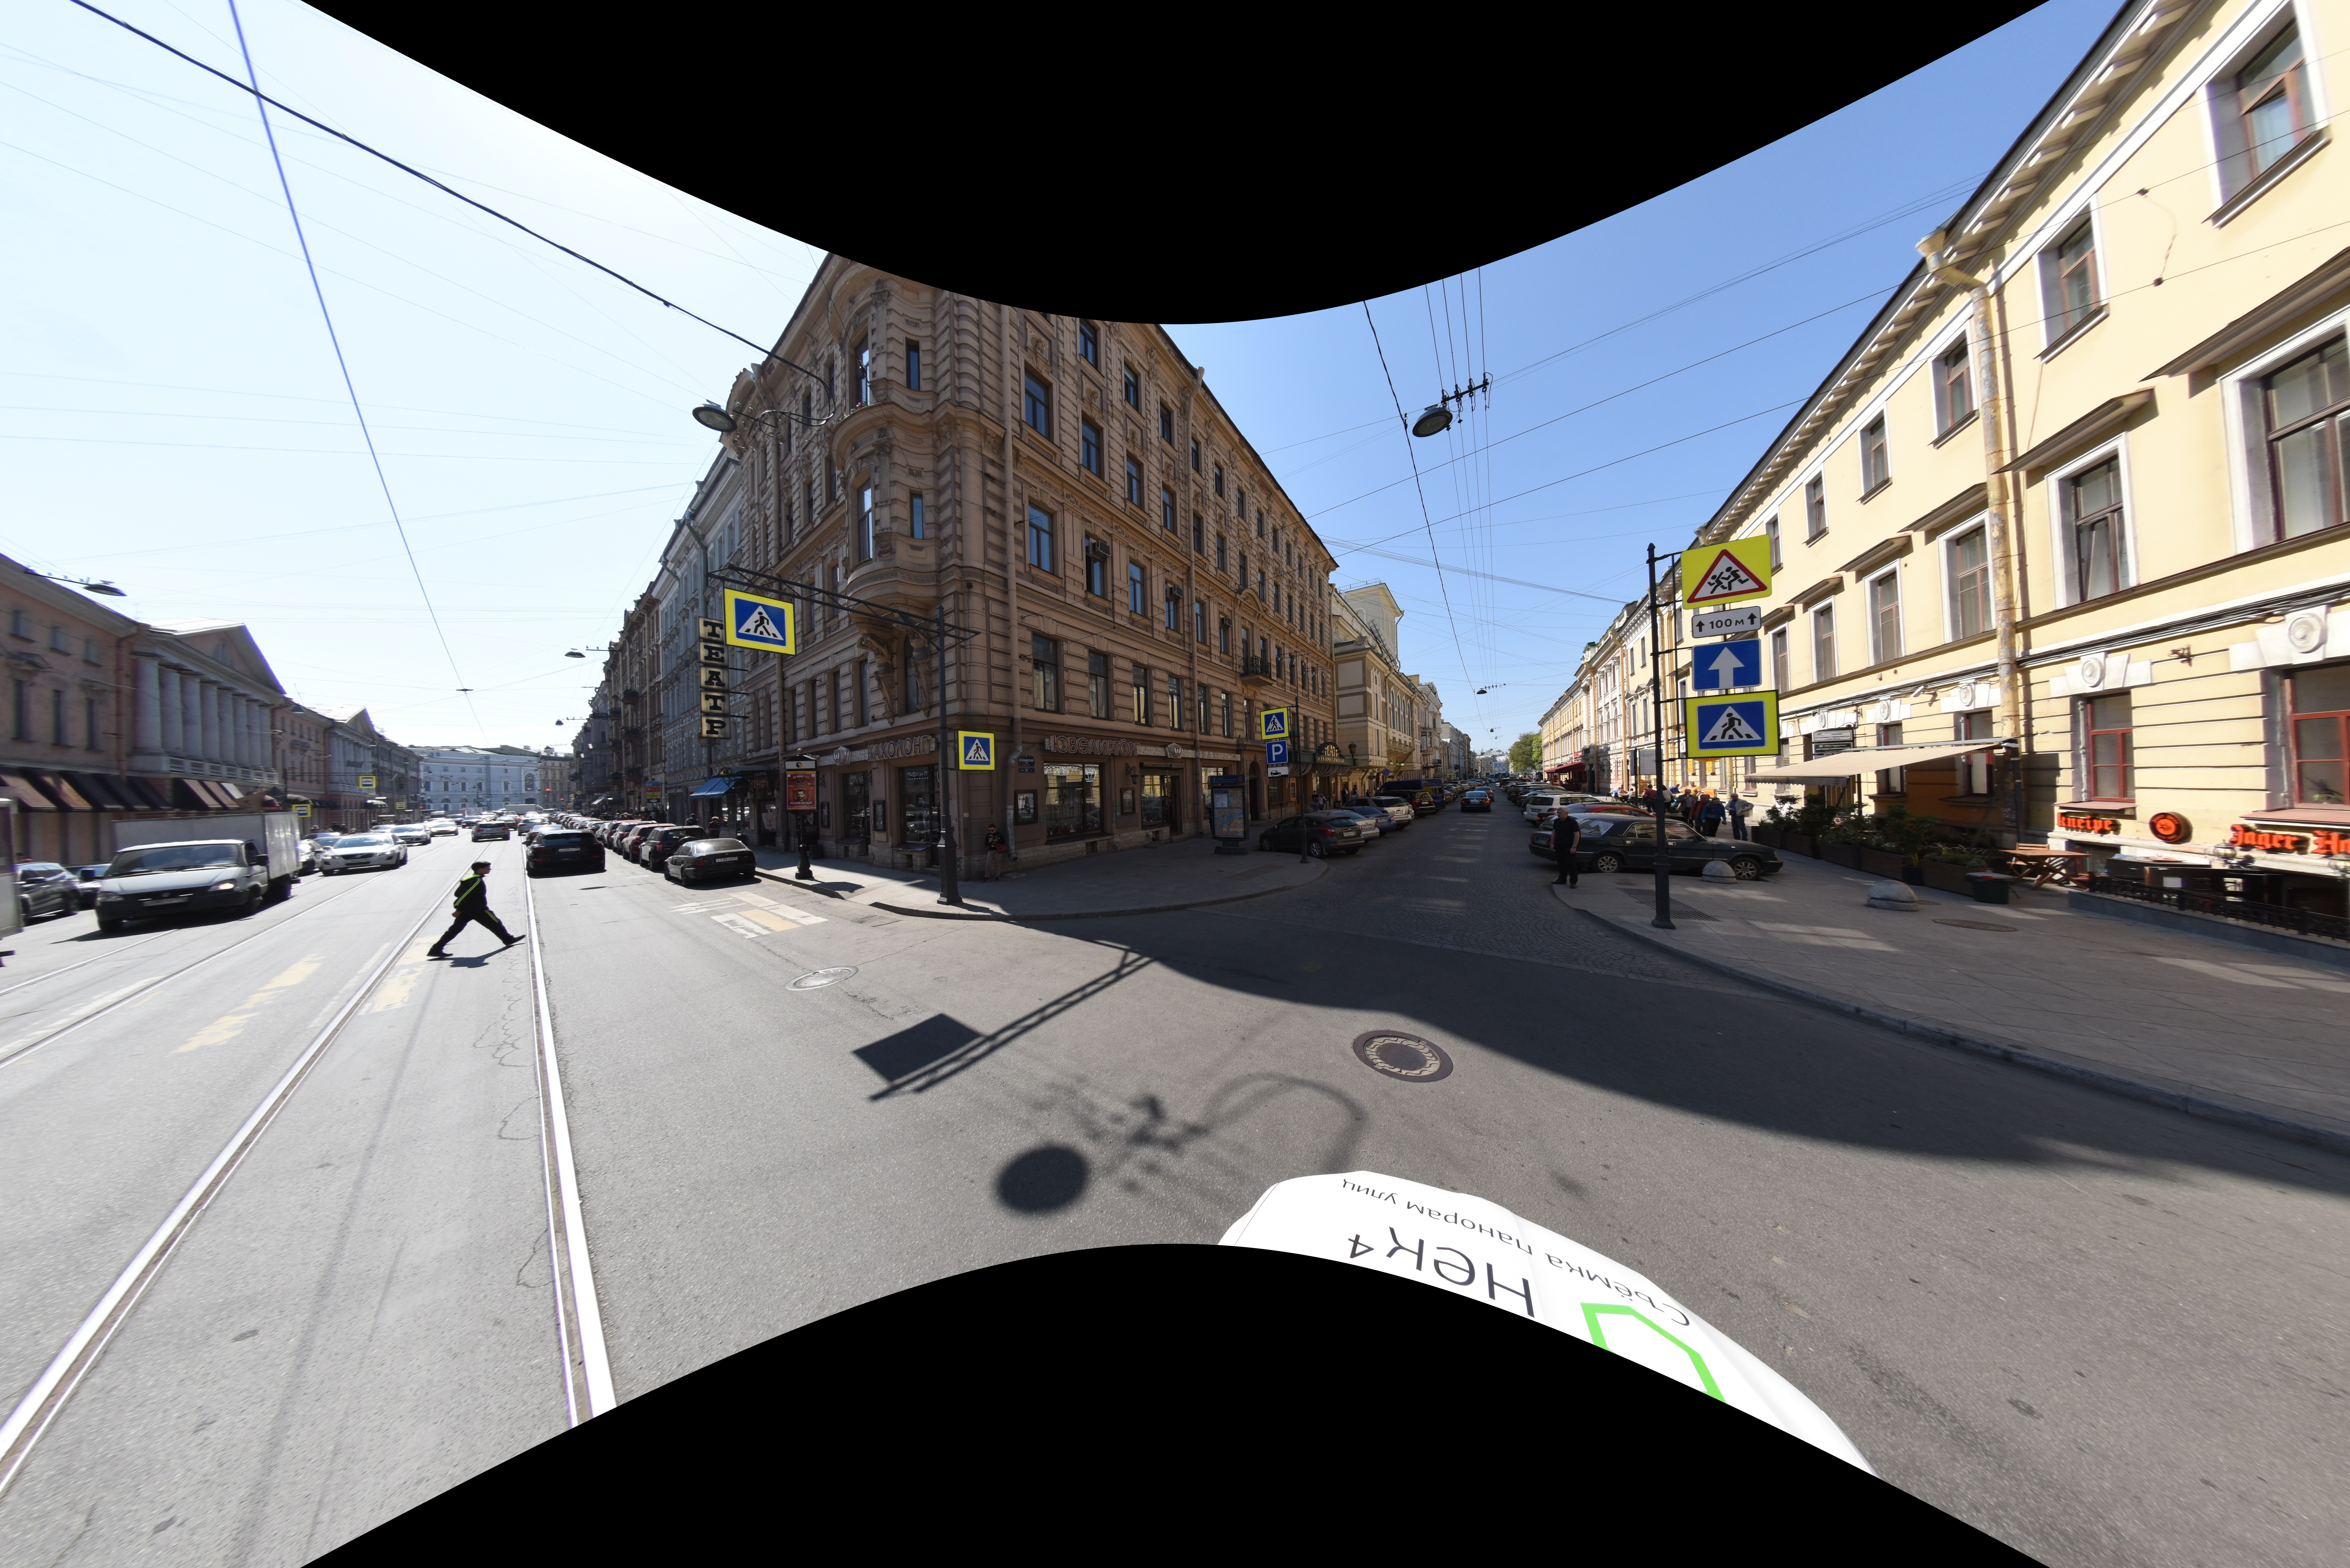
\includegraphics[width=0.9\textwidth]{figures/undistorted2A552.JPG}
	\caption{A552 с двумя коэффициентами после оптимизации}
\end{figure}
\begin{figure}[H]
	\centering 
	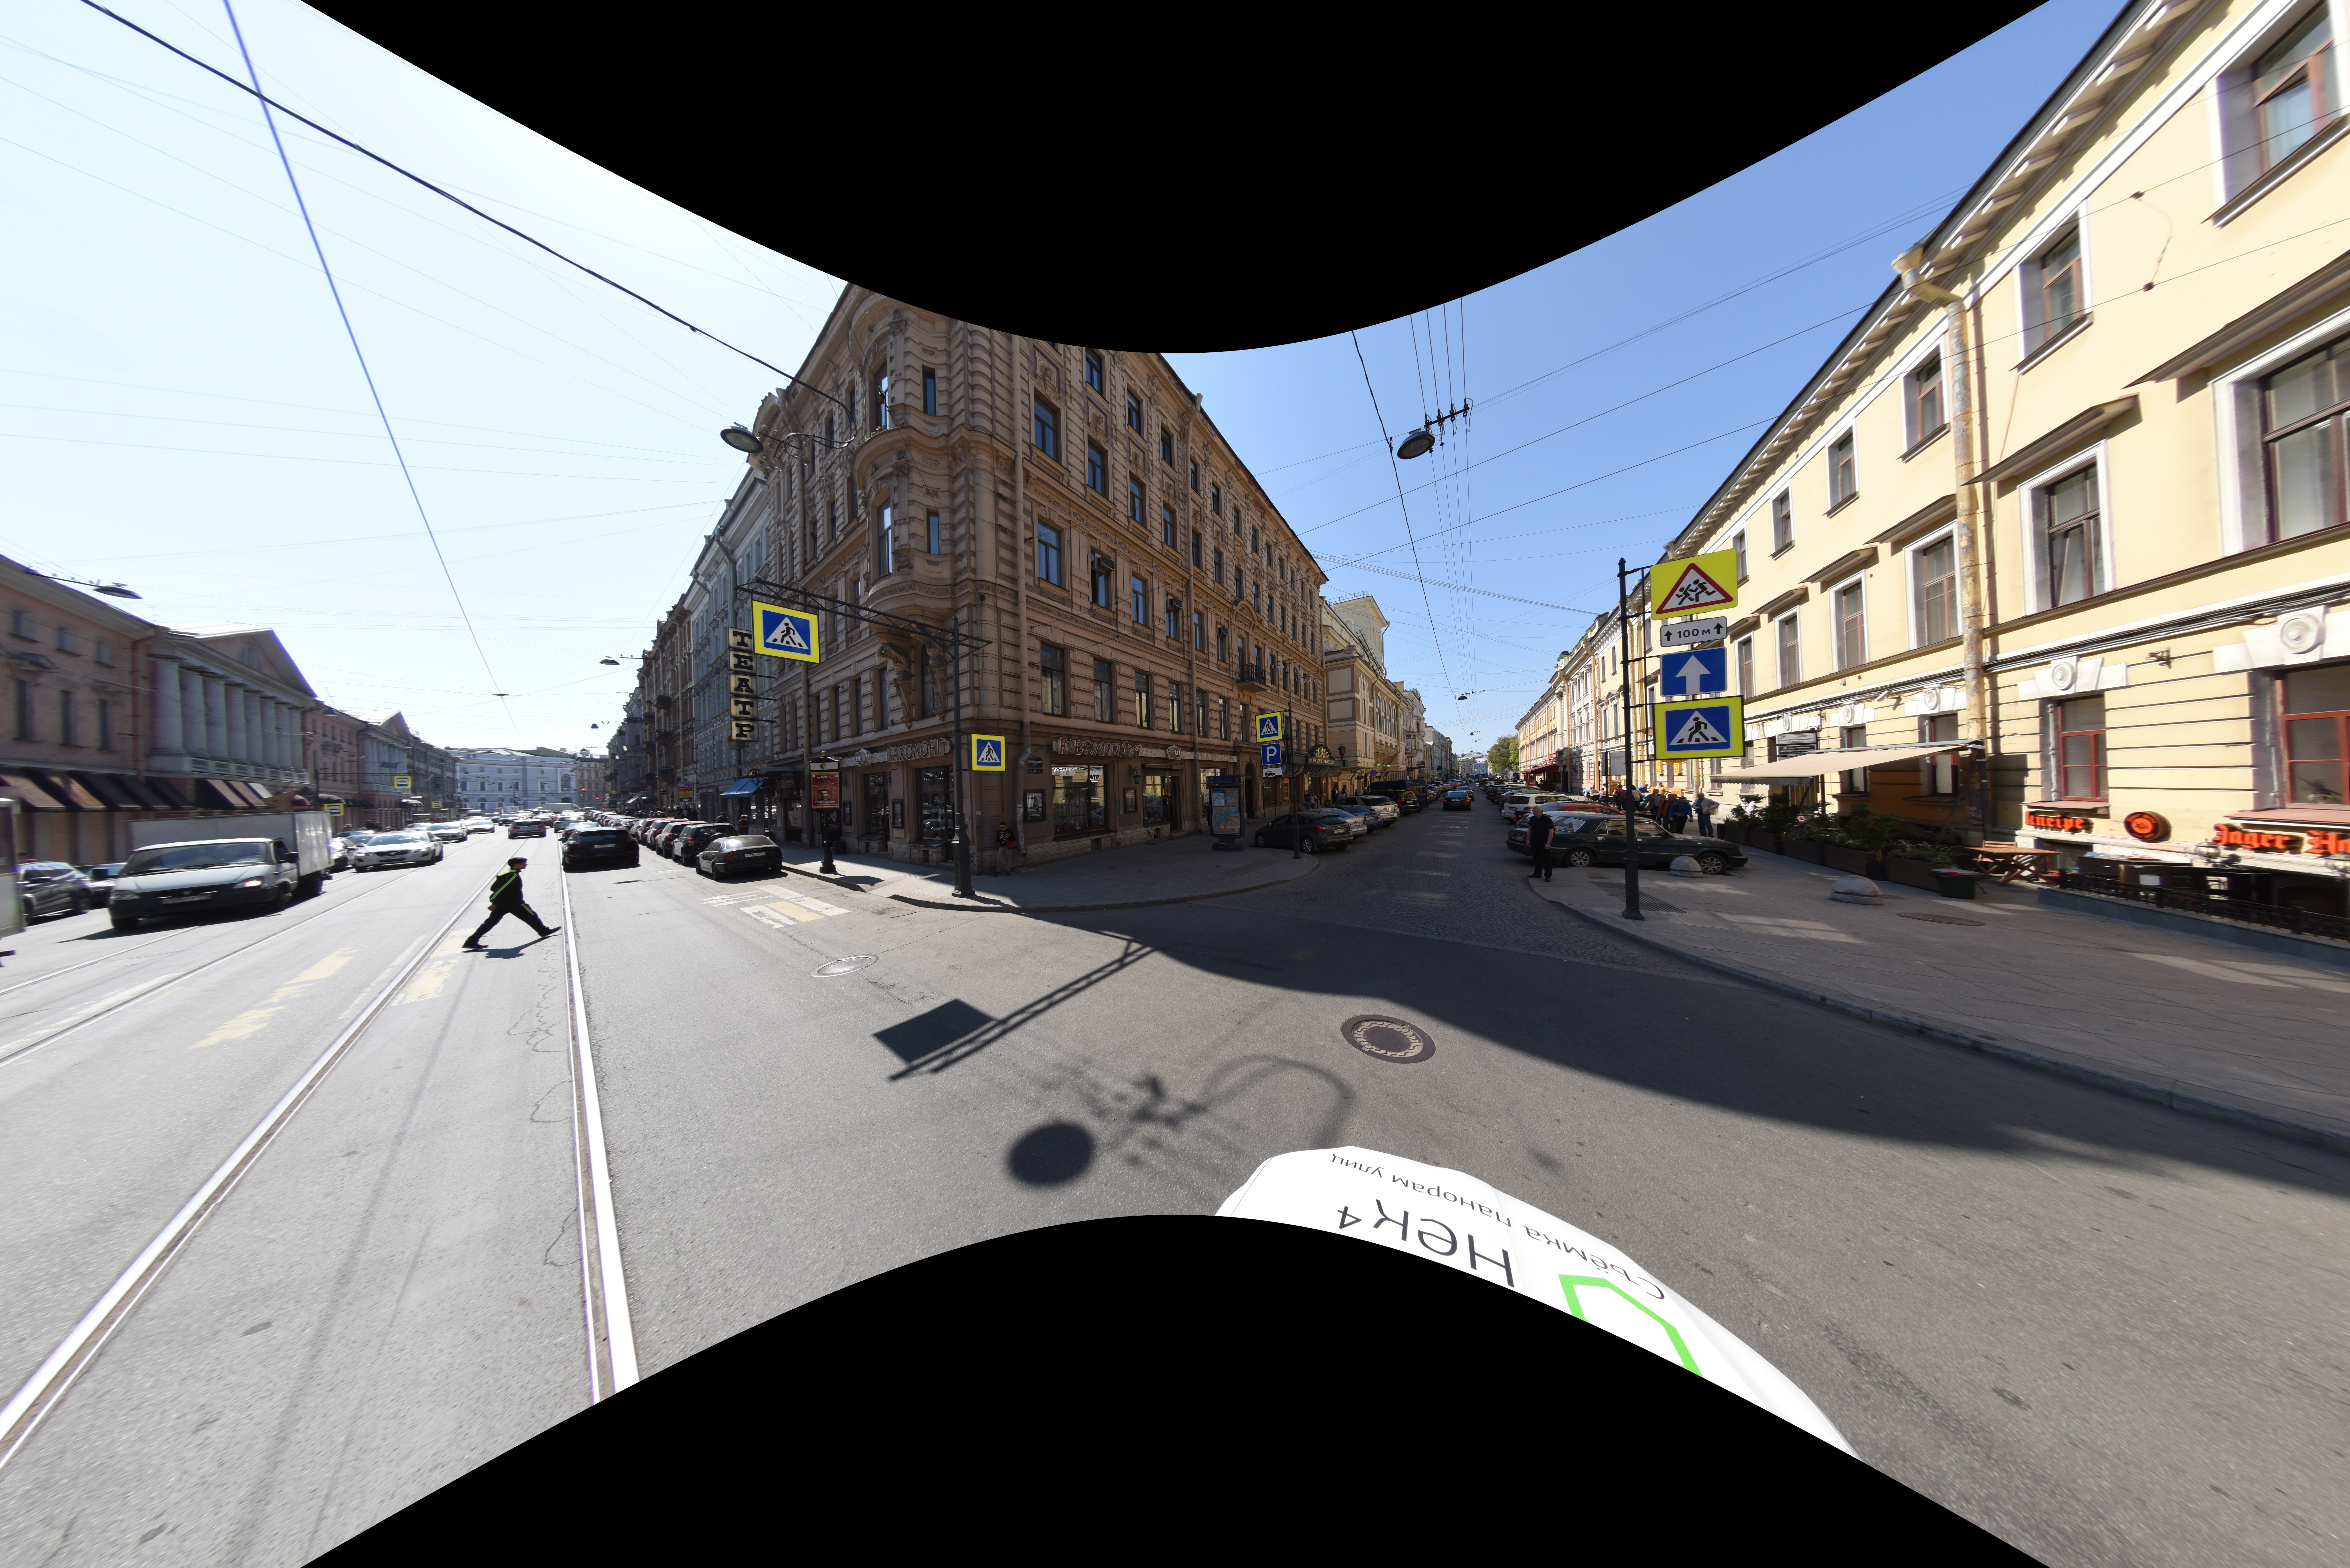
\includegraphics[width=0.9\textwidth]{figures/undistortedOp2A552.JPG}
	\caption{A552 с двумя коэффициентами после совместной оптимизации}
\end{figure}
\begin{figure}[H]
	\centering 
	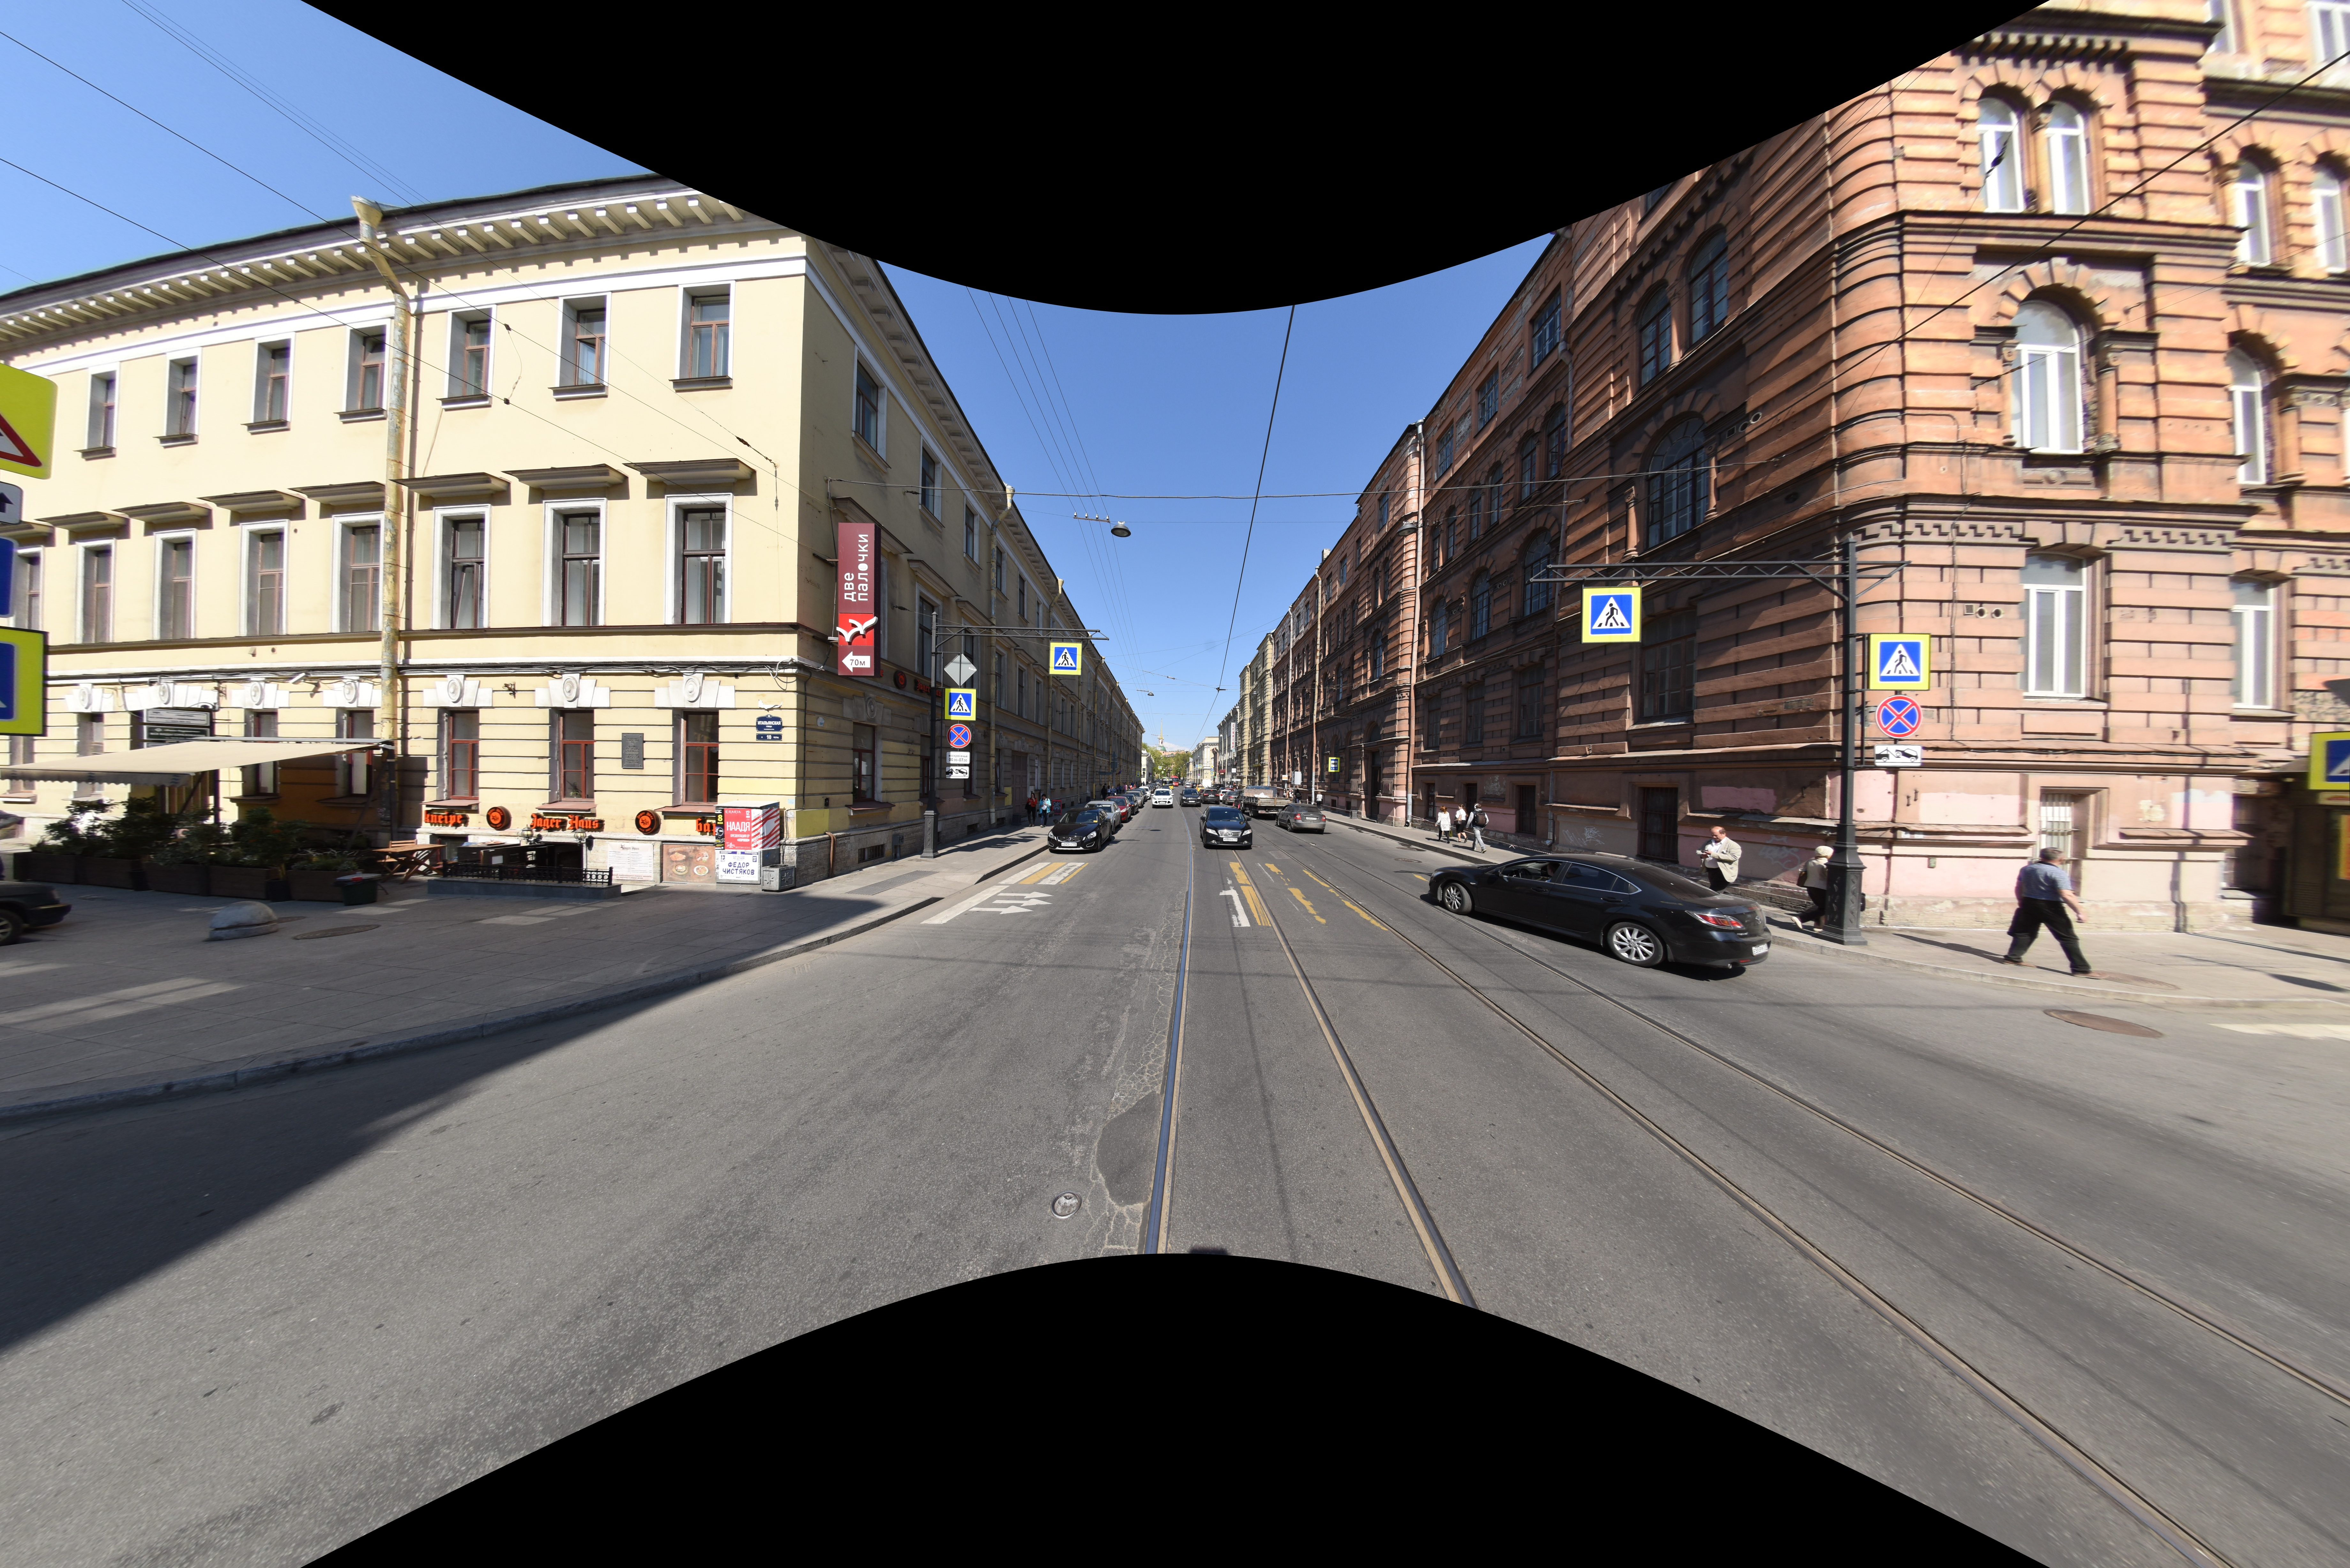
\includegraphics[width=0.9\textwidth]{figures/undistortedB552.JPG}
	\caption{B552 с одним коэффициентом}
\end{figure}
\begin{figure}[H]
	\centering 
	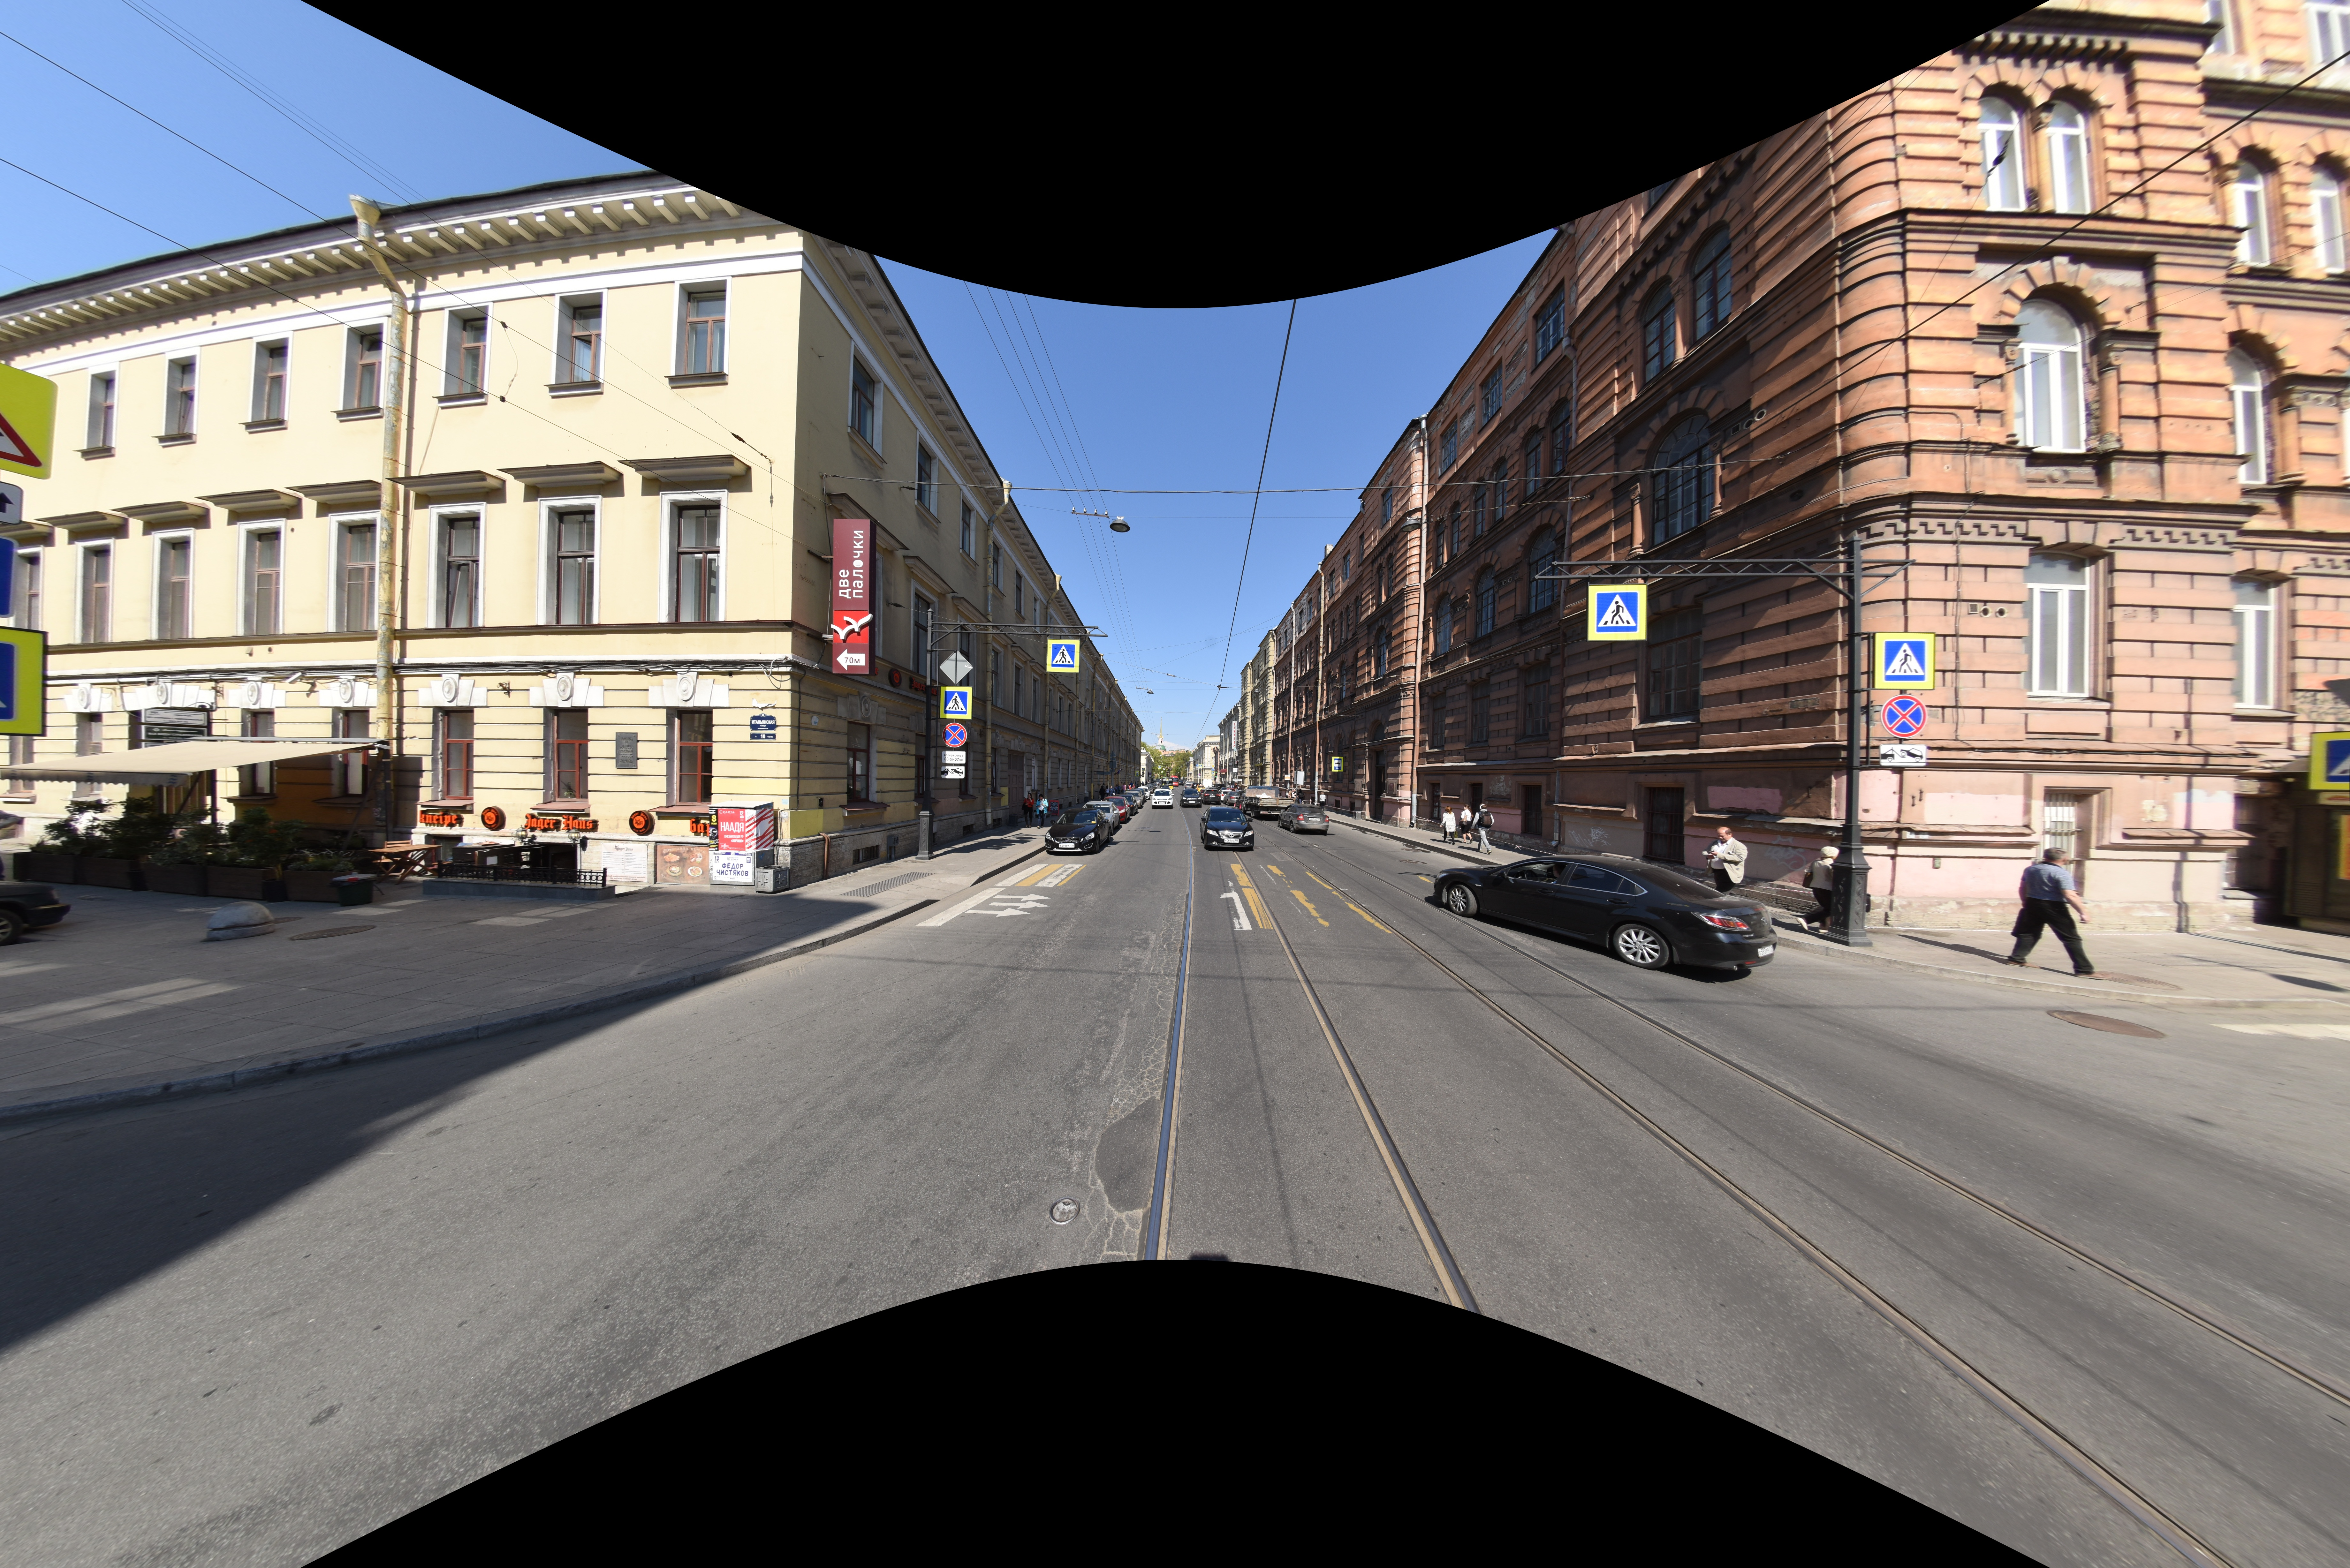
\includegraphics[width=0.9\textwidth]{figures/undistorted2B552.JPG}
	\caption{B552 с двумя коэффициентами после оптимизации}
\end{figure}
\begin{figure}[H]
	\centering 
	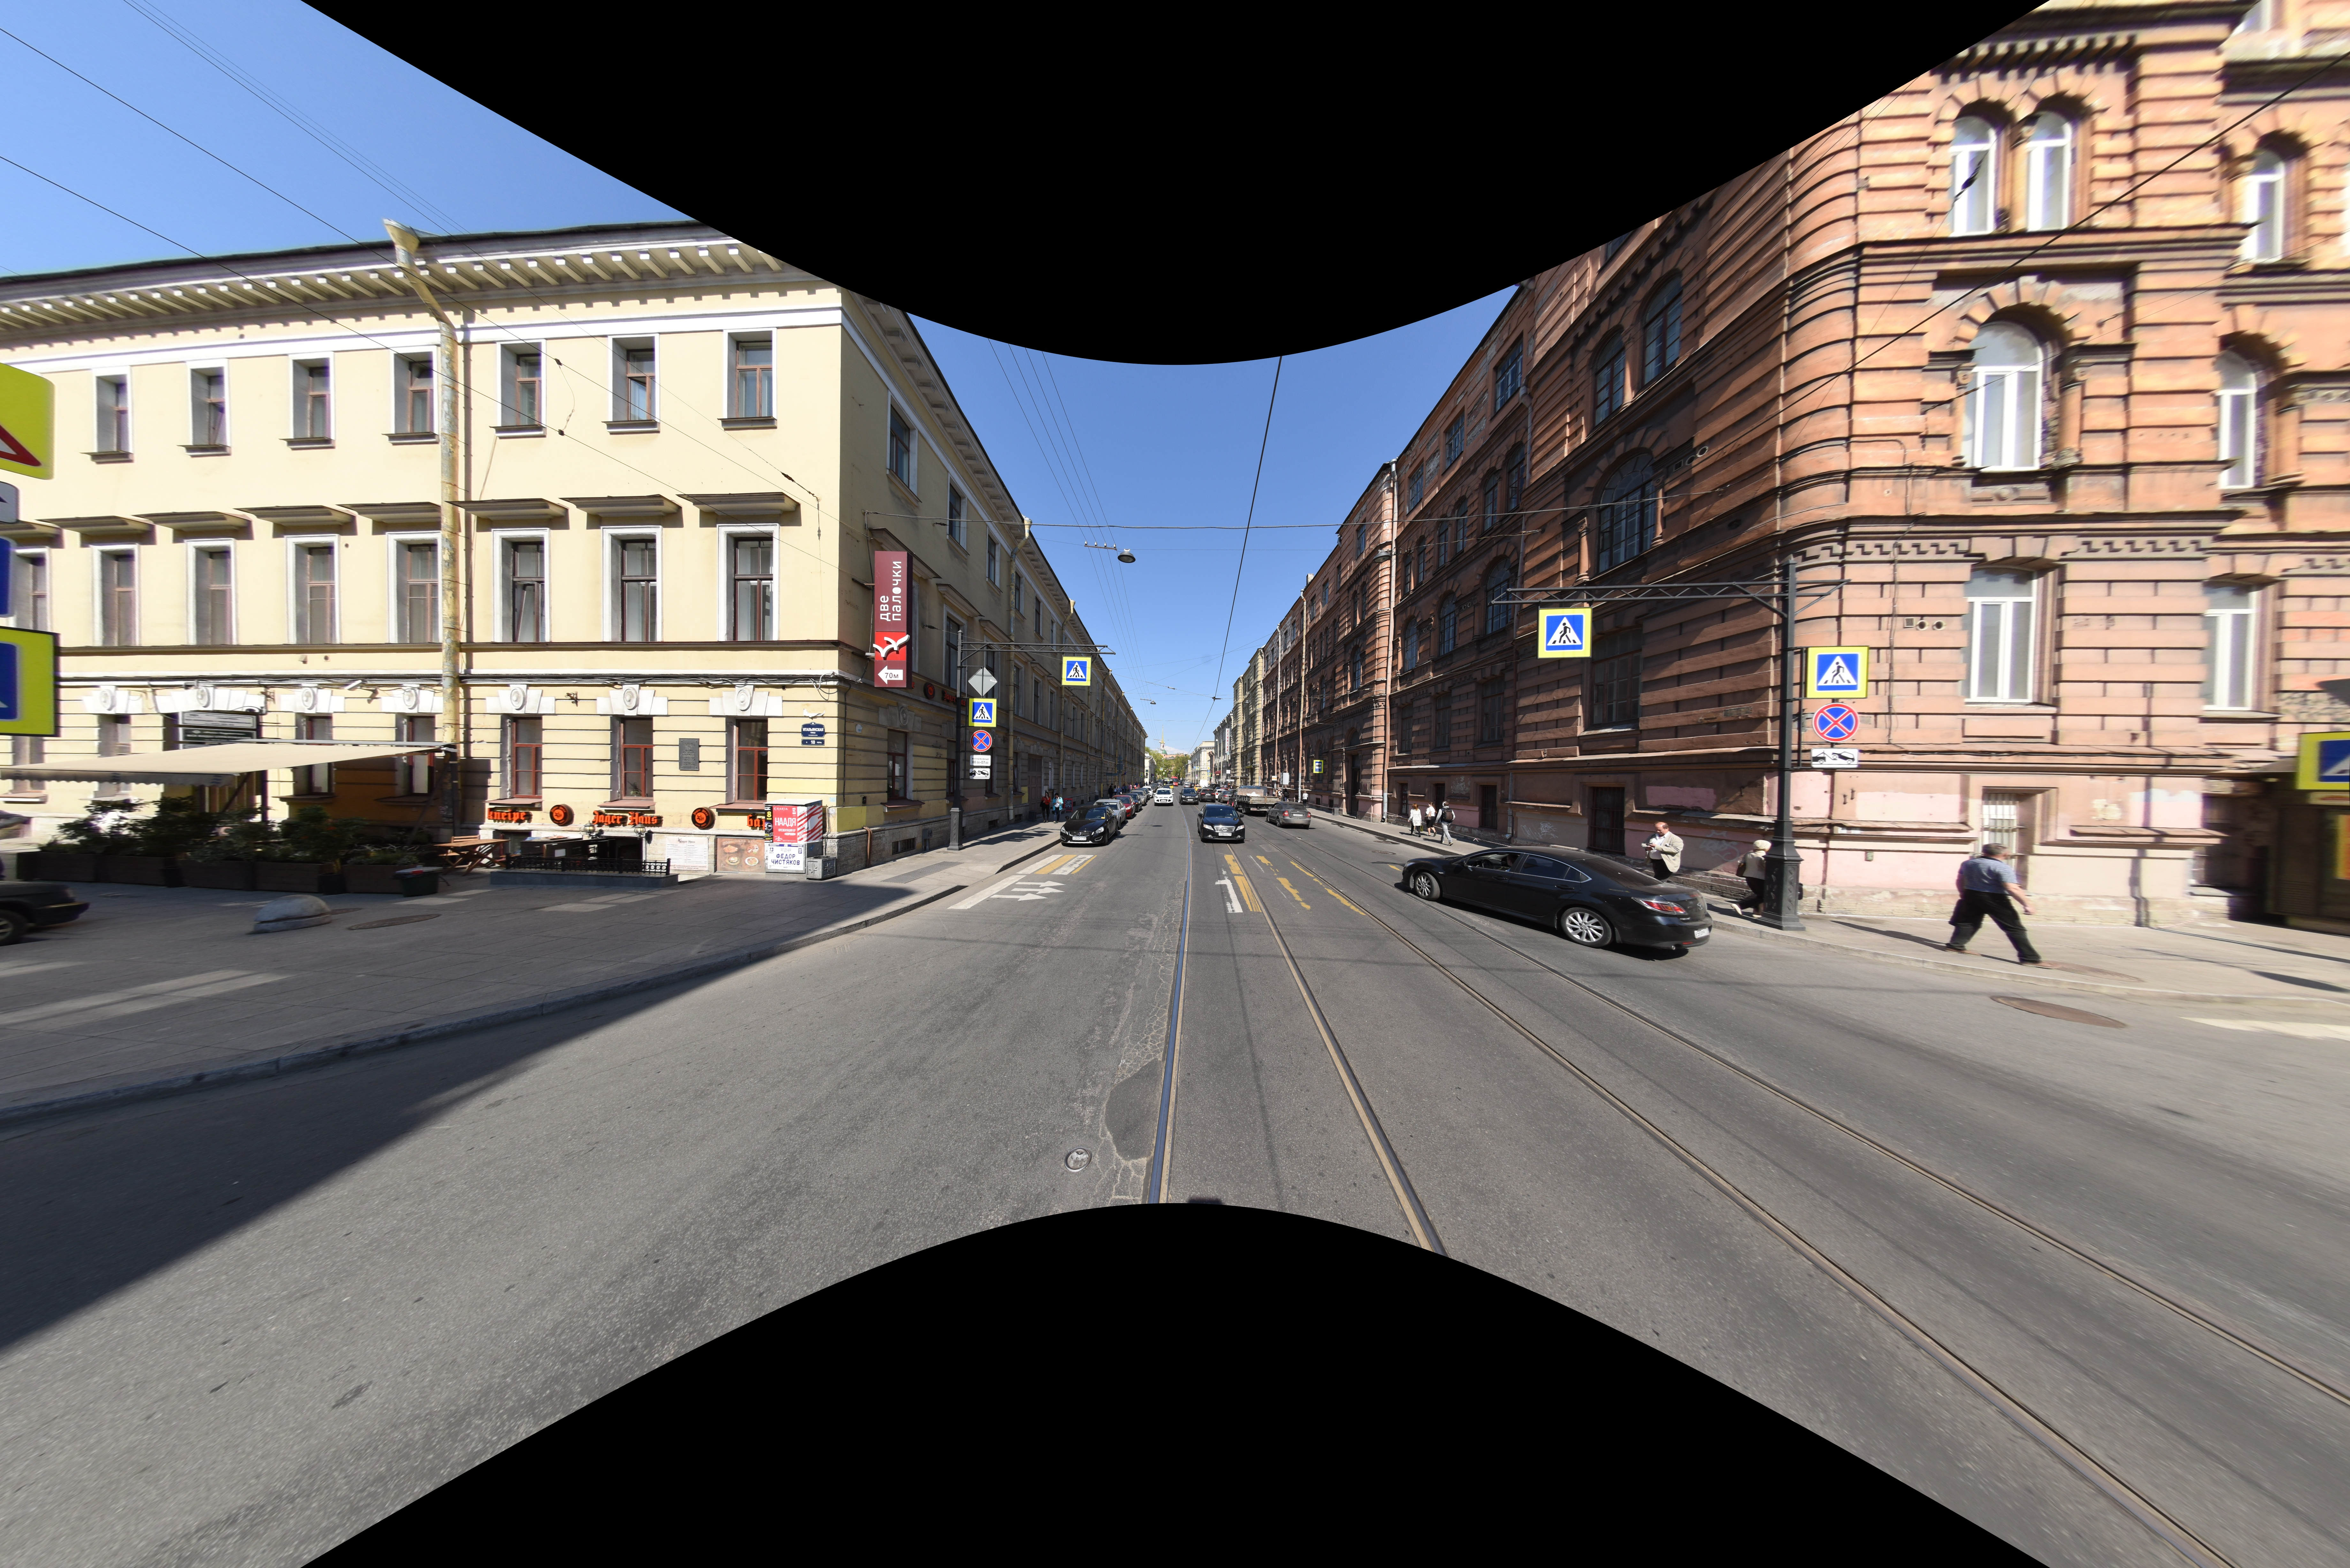
\includegraphics[width=0.9\textwidth]{figures/undistortedOp2B552.JPG}
	\caption{B552 с двумя коэффициентами после совместной оптимизации}
\end{figure}
\begin{figure}[H]
	\centering 
	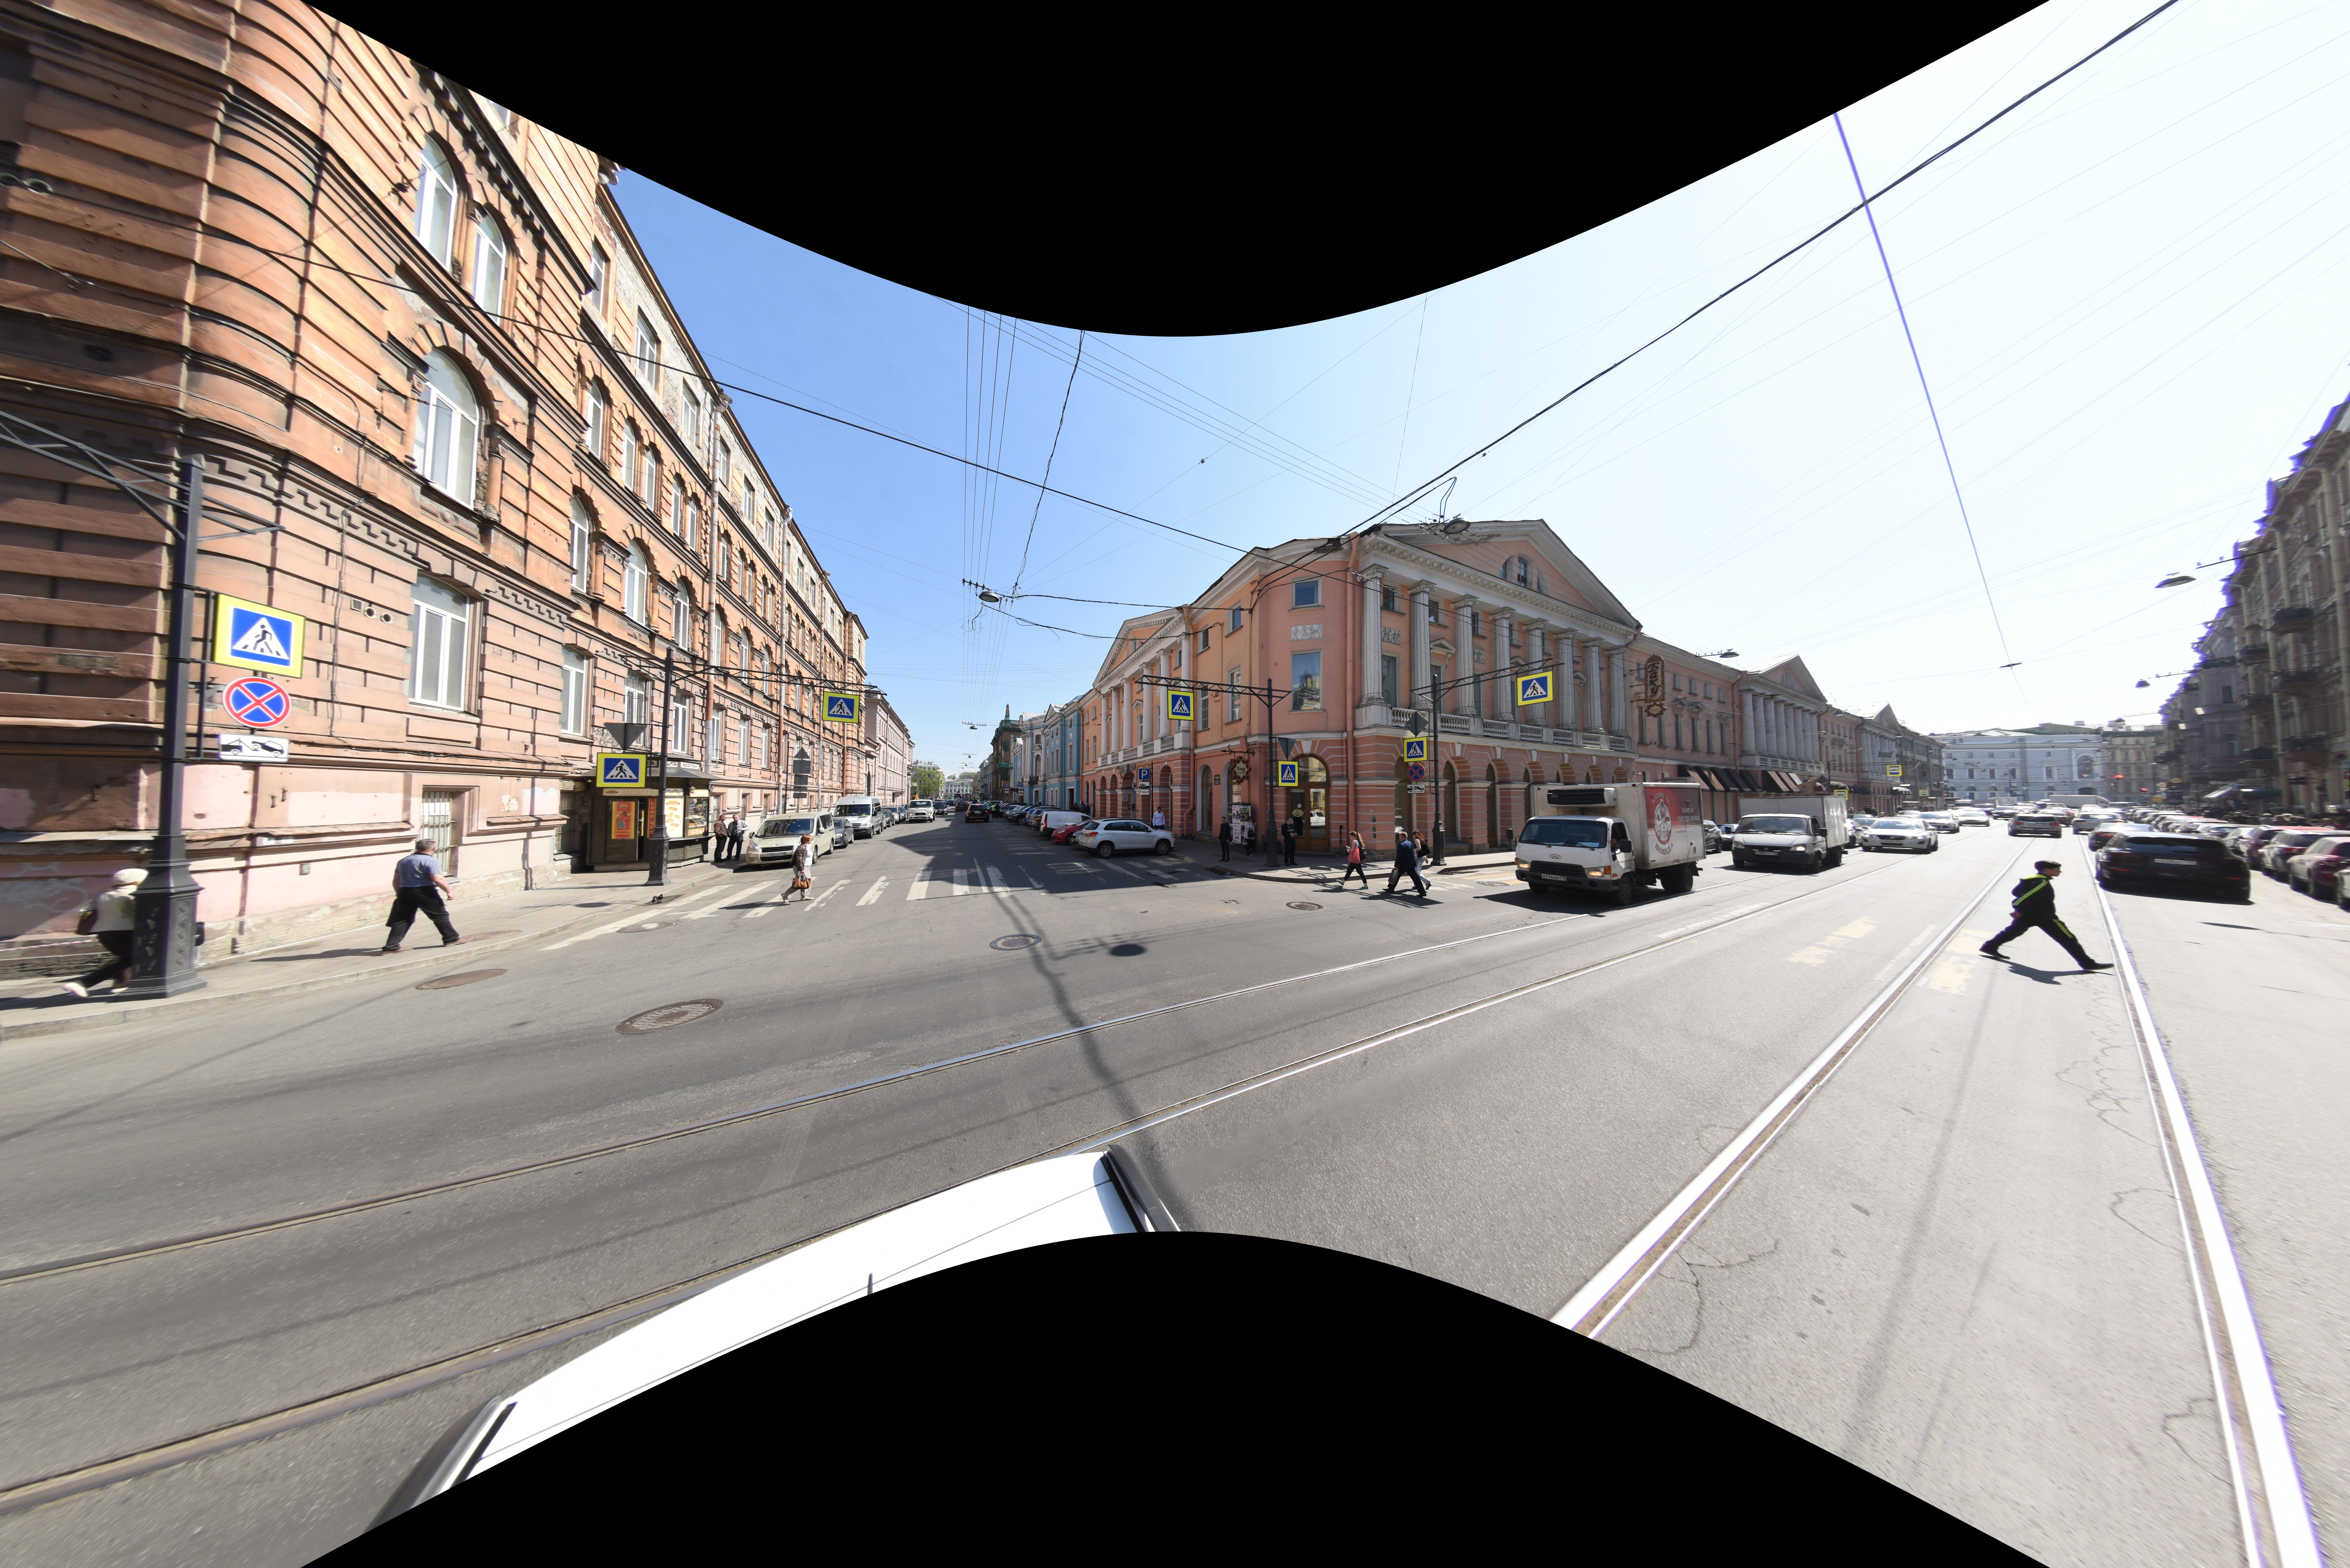
\includegraphics[width=0.9\textwidth]{figures/undistortedC552.JPG}
	\caption{C552 с одним коэффициентом}
\end{figure}
\begin{figure}[H]
	\centering 
	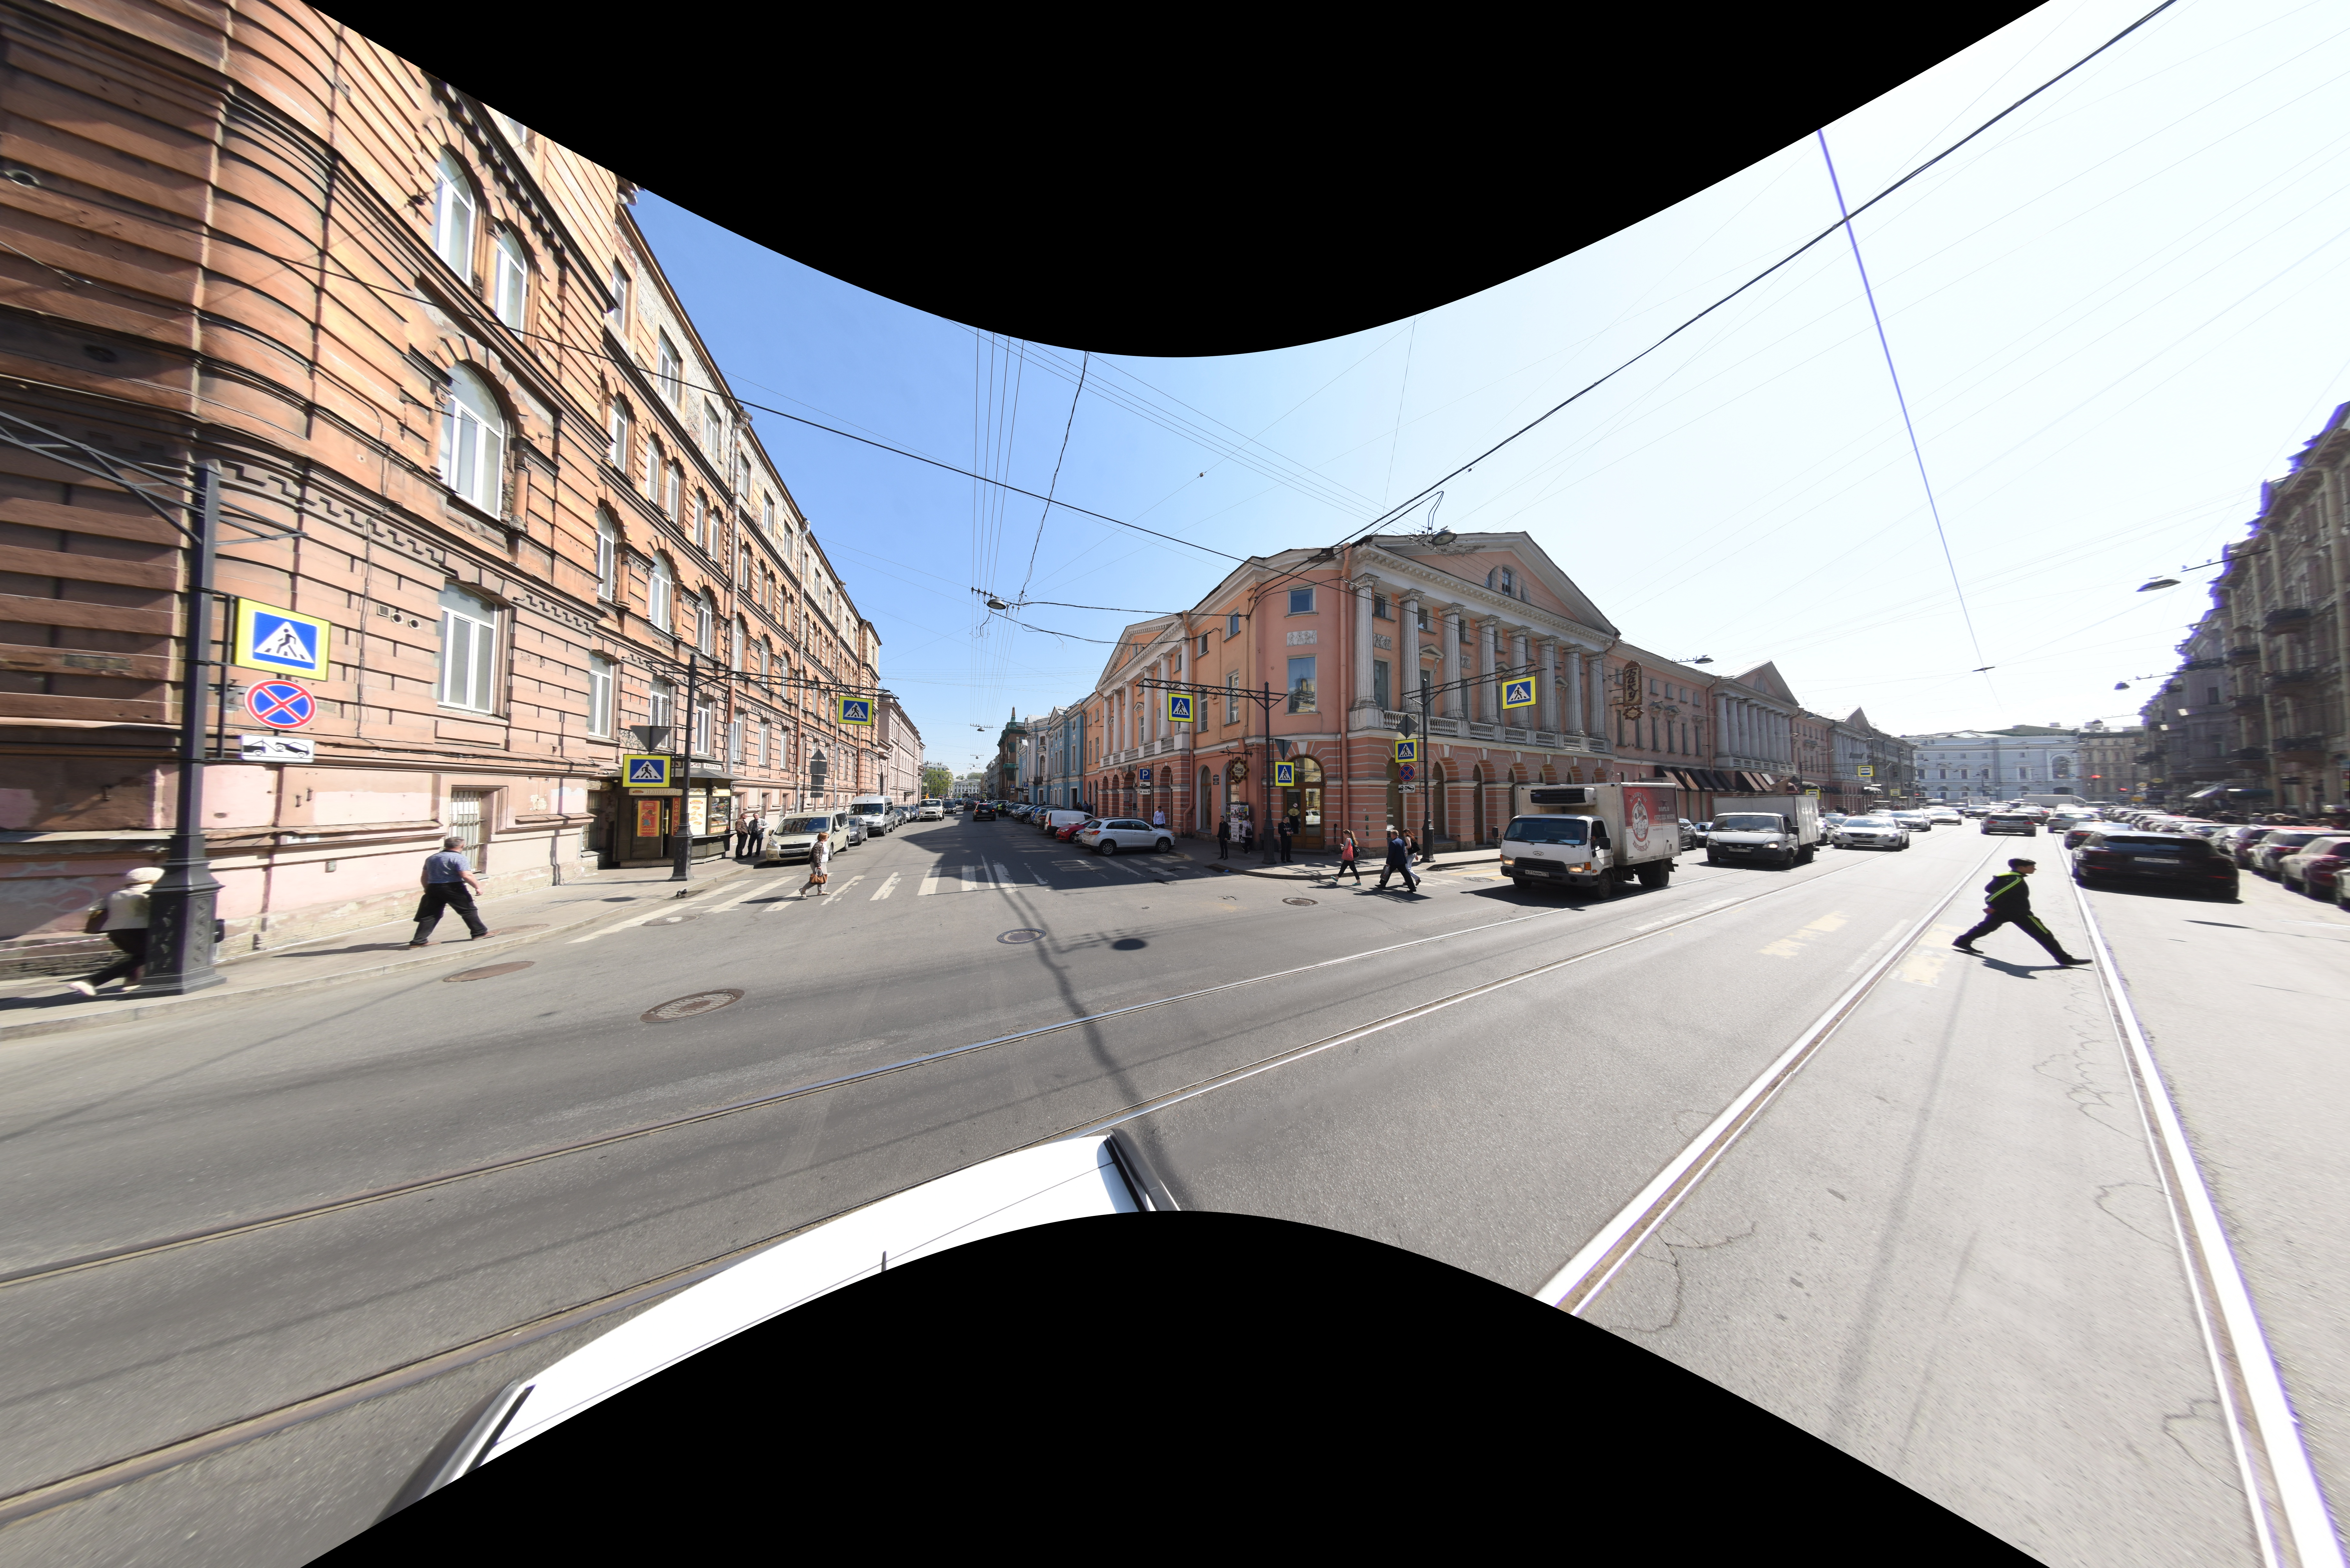
\includegraphics[width=0.9\textwidth]{figures/undistorted2C552.JPG}
	\caption{C552 с двумя коэффициентами после оптимизации}
\end{figure}
\begin{figure}[H]
	\centering 
	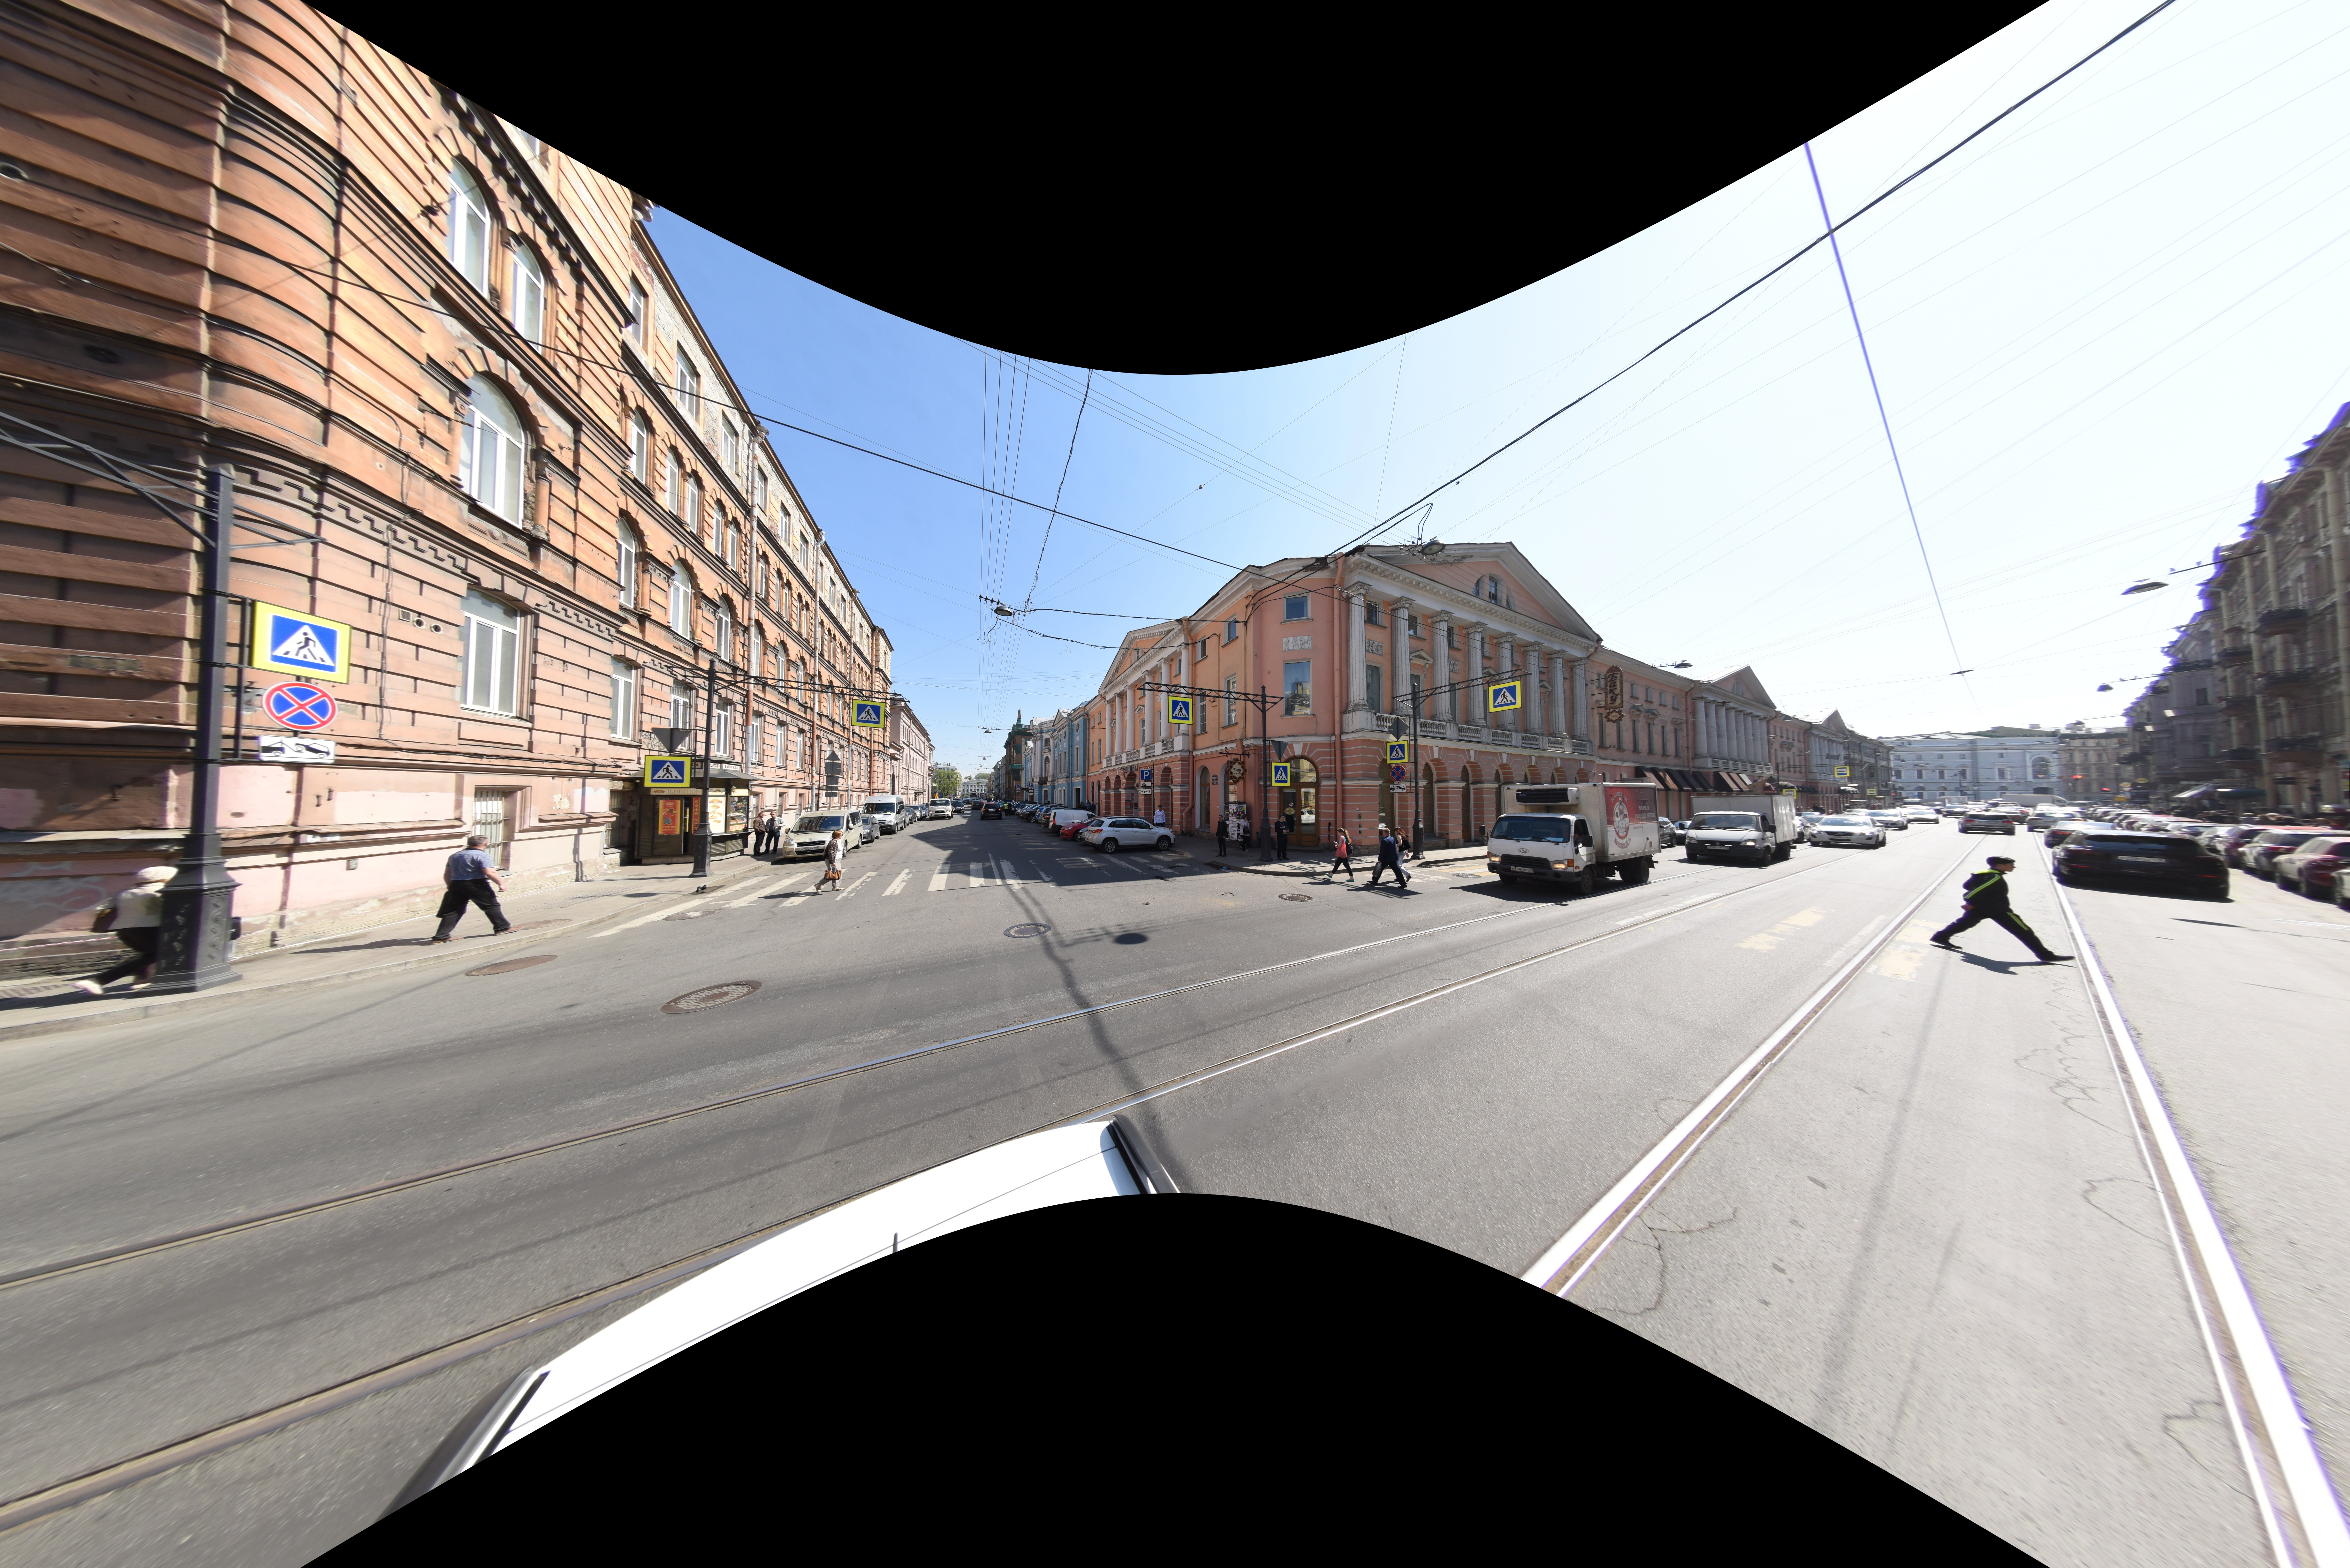
\includegraphics[width=0.9\textwidth]{figures/undistortedOp2C552.JPG}
	\caption{C552 с двумя коэффициентами после совместной оптимизации}
\end{figure}

\section{Оценки фундаментальных матриц}
Далее представлены изображения с частью инлаеров и эпиполярными линиями.

\begin{figure}[H]
	\centering 
	\includegraphics[width=0.9\textwidth]{figures/epilines_552_553.eps}
	\caption{Движение A552-A553 с двумя коэффициентами после совместной оптимизации}
\end{figure}
\begin{figure}[H]
	\centering 
	\includegraphics[width=0.9\textwidth]{figures/epilines_553_554.eps}
	\caption{Движение A553-A554 с двумя коэффициентами после совместной оптимизации}
\end{figure}
\begin{figure}[H]
	\centering 
	\includegraphics[width=0.9\textwidth]{figures/epilines_553_554_zoomed.eps}
	\caption{Увеличенный фрагмент A553-A554 с двумя коэффициентами после совместной оптимизации}
\end{figure}
\begin{figure}[H]
	\centering 
	\includegraphics[width=0.9\textwidth]{figures/epilines_552_553_B.eps}
	\caption{Движение B552-B553 с двумя коэффициентами после совместной оптимизации}
\end{figure}
\begin{figure}[H]
	\centering 
	\includegraphics[width=0.9\textwidth]{figures/epilines_553_554_B.eps}
	\caption{Движение B553-B554 с двумя коэффициентами после совместной оптимизации (красным отмечены примеры плохих соответствий, они получаются из-за того, что фичи на здании очень похожи)}
\end{figure}
\begin{figure}[H]
	\centering 
	\includegraphics[width=0.9\textwidth]{figures/epilines_552_553_C.eps}
	\caption{Движение C552-B553 с двумя коэффициентами после совместной оптимизации}
\end{figure}
\section{Оценки фокусных расстояний}
\begin{table}[H]
	\centering
	\begin{tabular}{| c | c | c | c | }
		\hline
		& DFOV & HFOV & VFOV \\ \hline
		A & 171 & 136 & 85 \\ \hline
		B & 175 & 147 & 98 \\ \hline
		C & 175 & 150 & 106 \\
		\hline
	\end{tabular}
	\caption{Оценки filed of view после совместной оптимизации}
\end{table}
\section{Оценки поз}
Траектория движения
\subsection{Примеры облаков триангулированных точек}
Облака точек